\documentclass[a0,landscape,pdftex]{a0poster}

\usepackage{amsthm,amsmath,amssymb,amsfonts,graphicx,algorithm,algorithmic}
\usepackage[scaled=1.1]{helvet}
\usepackage{postercols2}
\usepackage{flowfram}
\usepackage{color}
\usepackage{lipsum}
\usepackage{rotating}
\usepackage{subcaption}
\usepackage{booktabs}
\usepackage{multirow}
\usepackage{multicol}
\usepackage{paper_commands}


\setlength{\flowframesep}{.2in}
\setlength\parindent{0pt}
\setlength{\vcolumnsep}{.5in}
\setlength{\columnsep}{\vcolumnsep}

\Ncolumntop{static}{2}{3in}
\setstaticframe{1}{label={title}}

\newlength\offset
\setlength{\offset}{18.5in}
\addtolength{\offset}{\vcolumnsep}
\computeflowframearea{2}
\addtolength{\ffareaheight}{-\offset}
%\setflowframe{2}{height=\ffareaheight}
\addtolength{\ffareaheight}{\vcolumnsep}
%\newstaticframe{\ffareawidth}{18.5in}{\ffareax}{\ffareaheight}[figures]
\setstaticframe{20}{clear}

%this puts borders on the frames
%\setallflowframes{border=plain}
%\setallstaticframes{border=plain}

% \title{Disentangling and Integrating Relational and Sensory Information in Transformer Architectures}
%\author{}
\date{}


\begin{document}

% \begin{staticcontents*}{title}
% \maketitle
% \end{staticcontents*}
\thispagestyle{empty}

\Large


\begin{minipage}{50cm}

\vskip-11cm
\section*{Relational games}
\begin{center}
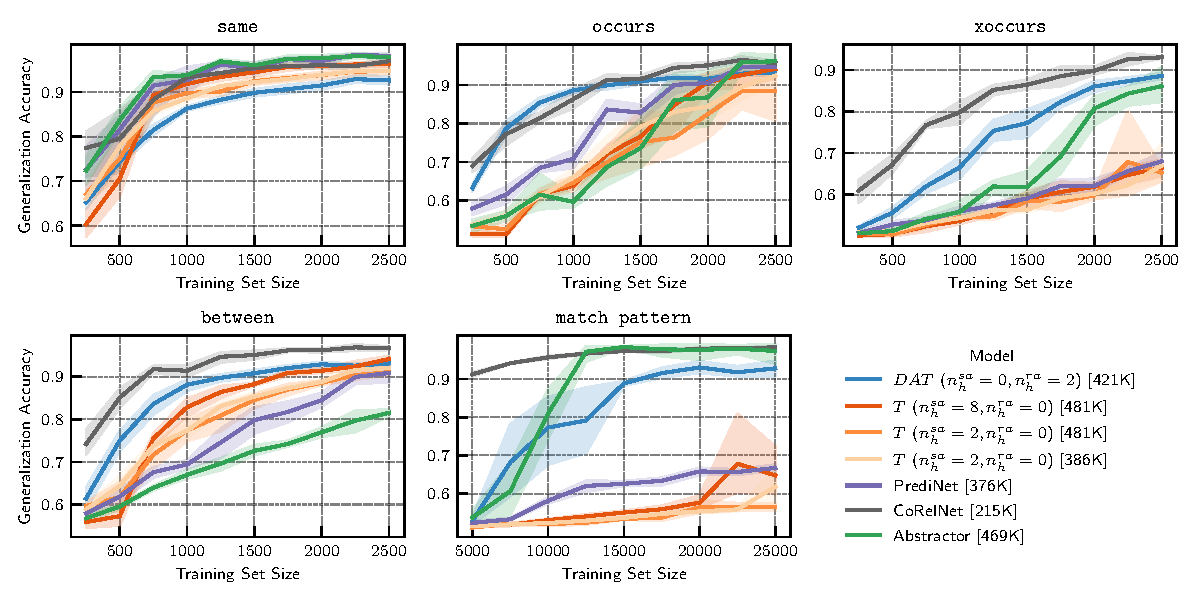
\includegraphics[width=\textwidth]{../figs/experiments/relgames/relgames_learning_curves_baseline_comparisons.pdf}
\end{center}
{\rm Figure 1. Learning curves on relational games, comparing \textit{DAT} against multiple Transformer baselines of varying sizes and architectural hyperparameters (e.g., \# of heads) as well as relational architecture baselines (PrediNet, CoRelNet, and Abstractor).}
\vskip2cm


\section*{Mathematical Symbolic processing}
% maybe pick one of the two 
% 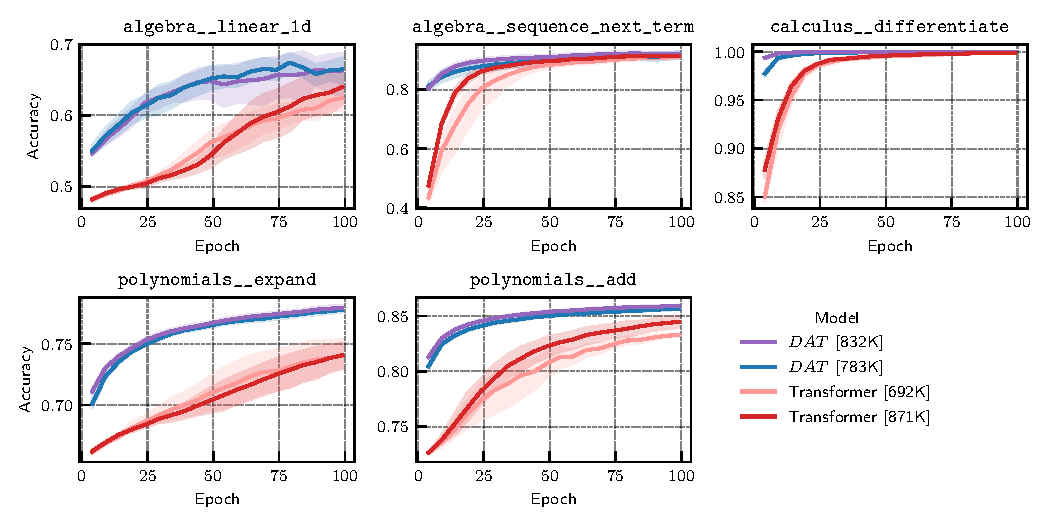
\includegraphics[width=0.95\textwidth]{../figs/experiments/math/math_training_curves_interpolation.pdf}

\begin{center}
    % \caption{Sequence-to-sequence symbolic mathematical processing. Comparison to Transformer at multiple scales. \textit{DAT} models have model dimension $128$ and Transformer models have model dimension $144$, with three models each with 2, 3, or 4 layers. Superiority of \textit{DAT} persists across all depths and model sizes.}
    {\normalsize
    \begin{tabular}{l|l|cc}
\toprule
Task & Model &  Accuracy \\
\midrule
\multirow{7}{*}{$\texttt{algebra\_\_linear\_1d}$} & Transformer [692K] &                    62.5\% \\
                                 & $DAT$ [783K] &                    66.5\% \\
                                 & Transformer [871K] &                    64.0\% \\
                                 & $DAT$ [1.09M] &                    76.6\% \\
                                 & Transformer [1.3M] &                    64.3\% \\
                                 & $DAT$ [1.43M] &                    74.7\% \\
                                 & Transformer [1.7M] &                    50.9\% \\
\cline{1-3}
\multirow{7}{*}{$\texttt{algebra\_\_sequence\_next\_term}$} & Transformer [692K] &                    91.1\% \\
                                 & $DAT$ [783K] &                    91.6\% \\
                                 & Transformer [871K] &                    91.4\% \\
                                 & $DAT$ [1.09M] &                    97.3\% \\
                                 & Transformer [1.3M] &                    96.9\% \\
                                 & $DAT$ [1.43M] &                        -- \\
                                 & Transformer [1.7M] &                    82.6\% \\
\cline{1-3}
\multirow{7}{*}{$\texttt{calculus\_\_differentiate}$} & Transformer [692K] &                    99.9\% \\
                                 & $DAT$ [783K] &                   100.0\% \\
                                 & Transformer [871K] &                    99.9\% \\
                                 & $DAT$ [1.09M] &                        -- \\
                                 & Transformer [1.3M] &                    99.9\% \\
                                 & $DAT$ [1.43M] &                   100.0\% \\
                                 & Transformer [1.7M] &                   100.0\% \\
\cline{1-3}
\multirow{7}{*}{$\texttt{polynomials\_\_add}$} & Transformer [692K] &                    83.3\% \\
                                 & $DAT$ [783K] &                    85.6\% \\
                                 & Transformer [871K] &                    84.5\% \\
                                 & $DAT$ [1.09M] &                    87.9\% \\
                                 & Transformer [1.3M] &                    86.9\% \\
                                 & $DAT$ [1.43M] &                    88.7\% \\
                                 & Transformer [1.7M] &                    87.3\% \\
\cline{1-3}
\multirow{7}{*}{$\texttt{polynomials\_\_expand}$} & Transformer [692K] &                    74.0\% \\
                                 & $DAT$ [783K] &                    77.8\% \\
                                 & Transformer [871K] &                    74.1\% \\
                                 & $DAT$ [1.09M] &                        -- \\
                                 & Transformer [1.3M] &                        -- \\
                                 & $DAT$ [1.43M] &                    92.2\% \\
                                 & Transformer [1.7M] &                    87.2\% \\
\bottomrule
\end{tabular}

    }
\end{center}
{\rm Table 1. Sequence-to-sequence symbolic mathematical processing. \textit{DAT} models have model dimension $128$ and Transformer models have model dimension $144$. Comparison across multiple scales with with 2, 3, or 4 layers.}

% {\rm Figure 2. Validation accuracy over the course of training for seq2seq mathematical problem-solving;
% number of parameters shown in brackets.}


\end{minipage}


\begin{minipage}{52cm}
\vskip -11cm
\section*{Language modeling at larger scale}

% 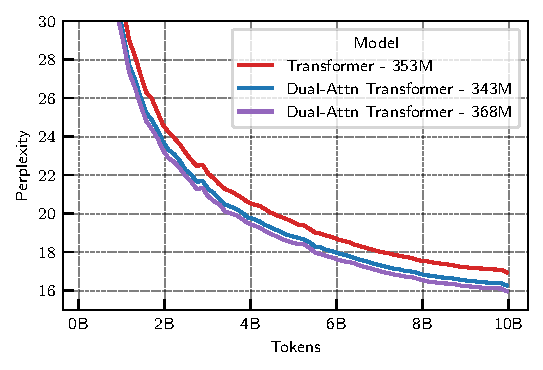
\includegraphics[width=.50\textwidth]{../figs/experiments/fineweb/350M_scale_lm.pdf}
% 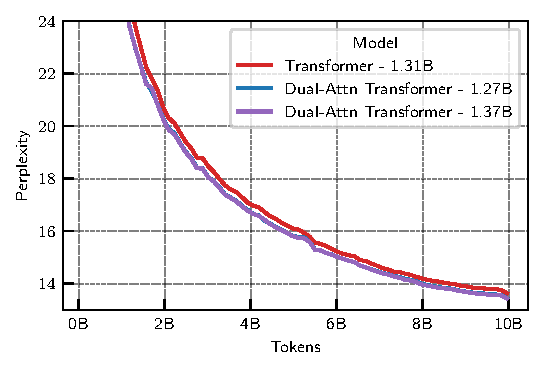
\includegraphics[width=.50\textwidth]{../figs/experiments/fineweb/1_3B_scale_lm.pdf}
\begin{center}
    % \begin{tabular}{@{}l|ccccccc|c@{}}
\begin{tabular}{@{}lcc|cccccc|c@{}}
    \toprule
    Model        & Param count   & \# Tokens &$\dmodel$&$\nlayers$& $\nhsa$  & $\nhra$ & $d_r$ & $n_{kv}^{h}$ & Perplexity $\downarrow$ \\ \midrule\hline
    Transformer  & 353M   & 10B       & 1024    & 24       & 16       & -        & -     & -           & 16.94     \\
    \textit{DAT} & 343M   & 10B       & 1024    & 24       & 8        & 8        & 8    & 4           & 16.26     \\
    \textit{DAT} & 343M   & 10B       & 1024    & 24       & 8        & 8        & 32    & 4           & 16.14     \\
    \textit{DAT} & 343M   & 10B       & 1024    & 24       & 8        & 8        & 64    & 4           & 16.09     \\
    % \textit{DAT} & 368M   & 10B       & 1024    & 24       & 8        & 8        & 8   & 8           & 15.97     \\\midrule
    Transformer  & 1.31B  & 10B       & 2048    & 24       & 32       & -        & -     & -           & 13.63     \\
    \textit{DAT} & 1.27B  & 10B       & 2048    & 24       & 16       & 16       & 64    & 8           & 13.44     \\
    \textit{DAT} & 1.37B  & 10B       & 2048    & 24       & 16       & 16       & 64    & -          & 13.43     \\ \bottomrule
    % Model / Param count   &$\dmodel$&$\nlayers$& $\nhsa$  & $\nhra$ & $n_r$ & $n_{kv}^{h}$ & Perplexity $\downarrow$ \\ \midrule\hline
    % Transformer - 353M   & 1024    & 24       & 16       & -        & -     & -           & 16.944     \\
    % \textit{DAT} - 343M  & 1024    & 24       & 8        & 8        & 32    & 4           & 16.258     \\
    % \textit{DAT} - 368M  & 1024    & 24       & 8        & 8        & 32    & 8           & 15.969     \\\midrule
    % Transformer - 1.31B  & 2048    & 24       & 32       & -        & -     & -           & 13.630     \\
    % \textit{DAT} - 1.27B & 2048    & 24       & 16       & 16       & 64    & 8           & 13.440     \\
    % \textit{DAT} - 1.37B & 2048    & 24       & 16       & 16       & 64    & 16          & 13.426     \\ \bottomrule
\end{tabular}%
    % }
    % & $n_s$ 
    % & -     
    % & 1024  
    % & 1024  
    % & -     
    % & 512   
    % & 2048  
\end{center}
{Table 2. Language modeling with the Fineweb dataset. Models up to 1.3B parameters in size are trained on 10B tokens of high-quality text data scraped from the internet. The \textit{DAT} model is superior to the corresponding Transformer at both the 350M scale and the 1.3B scale. We compare the Transformer baseline against a slightly larger and slightly smaller \textit{DAT} model, both of which are superior.}
% {Figure 3. Perplexity for language modeling with the Fineweb dataset, for different size models. The $x$-axis indicates the number of tokens and the $y$-axis is the validation perplexity. Left: Each model has 24 layers; Transformer has 16 sensory heads; DAT models have 8 sensory heads and 8 relational heads; relational heads have 32-dimensional relations. Right: Each model has 24 layers; Transformer has 32 sensory heads; DAT models have 16 sensory heads and 16 relational heads; relational heads have 64-dimensional relations.}

% \begin{minipage}{35cm}
\section*{Visualizing Learned Relational Attention Heads}
% \vskip3cm
{Figure 2. Visualization of learned attention heads in trained \textit{DAT} language models (343M \textit{DAT}-LM)}
\begin{center}

\begin{tabular}{lll}
    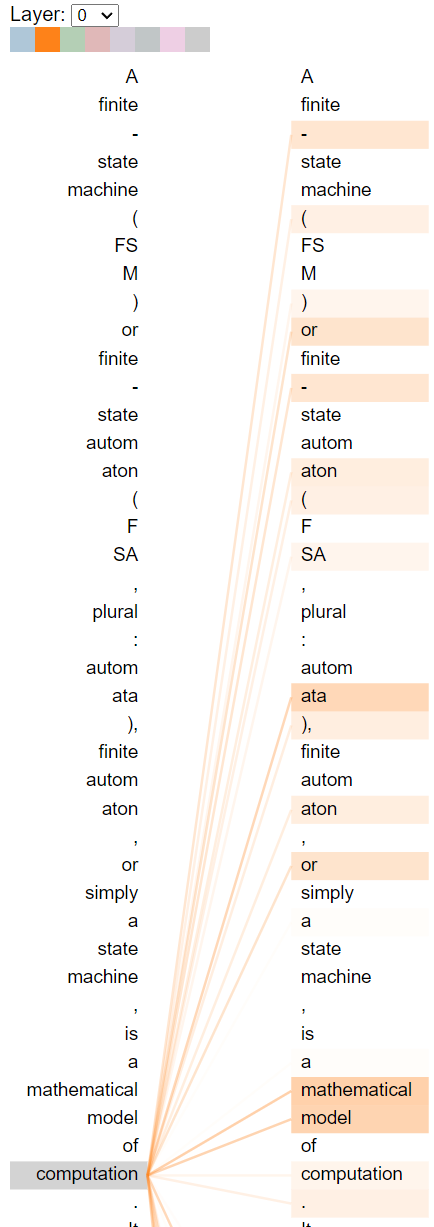
\includegraphics[width=.38\textwidth]{attn1} &
    \qquad \raisebox{-6.5cm}{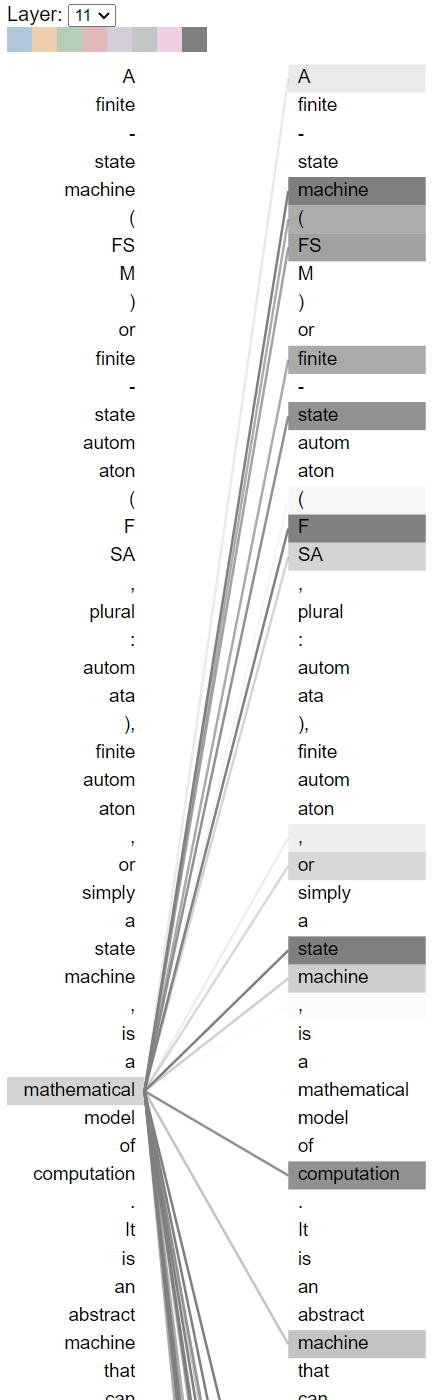
\includegraphics[width=.38\textwidth]{attn2}} &
    % \qquad 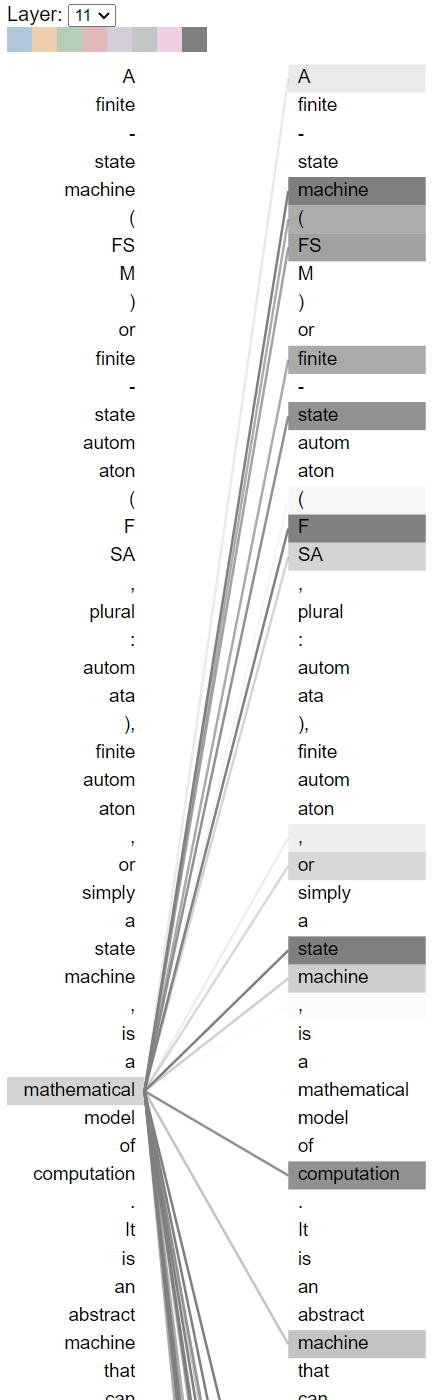
\includegraphics[width=.40\textwidth]{attn2} &
% \qquad \raisebox{40cm}{\begin{minipage}{25cm} Figure 4. Diagrams showing attention scores used by relational heads in two layers of a \sl{DAT} model trained on the Fineweb data. \end{minipage}}
\end{tabular}
\end{center}

% \vskip2cm

    % \vskip2cm

\end{minipage}


\end{document}
